\zerar
\chapter{Introdução}
\label{cap:introducao}

Métodos de otimização no planejamento das operações de uma empresa aérea têm sido aplicados a várias
décadas~\cite{yu}. Tal planejamento envolve diversos problemas que, devido ao tamanho e complexidade
de cada um, são normalmente resolvidos de forma separada e sequencial, embora alguns estejam
intimamente relacionados~\cite{barnhart03} (veja Figura~\ref{fig:planejamento}).

Primeiro, resolve-se o problema da \emph{malha de voos}, que consiste em determinar todos os trechos
a serem voados pela empresa num determinado período de tempo. O planejamento é basicamente feito em
termos de demanda de mercado.

Segundo, trata-se do problema da \emph{atribuição de frotas}. Nele, determina-se qual o tipo de
aeronave (tal como Boeing 737, Boeing 767, Airbus 320, etc) deve ser atribuído para efetuar cada
trecho da malha de voos. O objetivo é maximizar os lucros de venda, em função da demanda prevista e
do custo de se operar determinada frota em determinado trecho, sujeito à restrição de que todos os
voos da malha sejam cobertos com a frota disponível.

Terceiro, considera-se o problema do \emph{roteamento de aeronaves}, que envolve a escolha das
aeronaves de uma frota que vão realizar determinados voos, de forma que cada aeronave passe um tempo
adequado em aeroportos específicos, com a finalidade de serem revisadas pela manutenção. O objetivo
é maximizar os lucros, respeitando ainda a restrição de que todos os voos da frota sejam cobertos.

Finalmente, o problema de \emph{escalonamento de tripulantes} é resolvido. Tal problema foi um dos
primeiros a receber atenção significativa por parte da comunidade de pesquisa
operacional~\cite{arabeyre69}, sendo ainda um dos mais estudados. Isto porque, no transporte aéreo,
os custos com a tripulação representam a segunda maior parcela dos custos operacionais da empresa,
perdendo apenas para os custos com combustível. Para se ter uma ideia, o custo total com tripulação
excede 1,3 bilhões de dólares todo ano na Americam Airlines~\cite{anbil91a}. Hoje em dia, a
otimização no planejamento de escalas representa economia de cerca de 50 milhões de dólares anuais
para uma companhia de grande porte~\cite{barnhart03}.

\begin{figure}[htbp]
	\begin{center}
		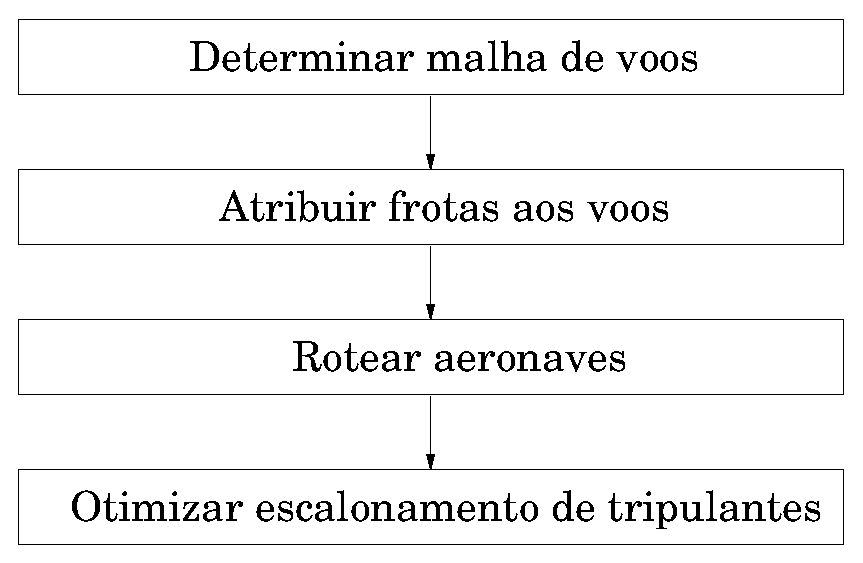
\includegraphics[scale=0.5]{fig/planejamento.eps}
		\caption{Sequência de problemas resolvidos no planejamento de operações de uma empresa
		aérea.}
		\label{fig:planejamento}
	\end{center}
\end{figure}

De forma geral, o escalonamento de tripulantes pode ser definido como o problema de se atribuir a um
grupo de trabalhadores (uma tripulação) um conjunto de atividades. No contexto da aviação, cada
tripulante (comandante, co-piloto, comissário, etc) deve ser designado para realizar um determinado
voo da empresa. Tal designação deve ser feita respeitando-se uma série de restrições impostas pelas
agências reguladoras da aviação, bem como regras de regulamentação trabalhista, restrições
operacionais impostas pela própria empresa e acordos trabalhistas entre empregado e empregador. Dado
o grande número de variáveis e restrições envolvidas, assim como a possibilidade de grandes ganhos
econômicos, o problema torna-se bastante interessante, tanto do ponto de vista da indústria, quanto
acadêmico.

Normalmente, o problema do escalonamento de tripulantes é dividido em dois subproblemas que são
resolvidos de forma independente e sequencial. O primeiro deles é conhecido como \emph{problema da
determinação de viagens} (PDV), que consiste na obtenção de um subconjunto de viagens, obedecendo as
regras de trabalho impostas pela legislação, com custo mínimo, cobrindo todas os segmentos de voo
exatamente uma vez. Obtida a solução das viagens, um segundo problema é resolvido, conhecido como
\emph{problema da determinação de escalas} (PDE), cujo objetivo é construir as escalas dos
tripulantes, distribuindo as viagens de tal forma que cada viagem seja atribuída exatamente uma vez
para cada tripulante necessário. Na atribuição, visa-se minimizar os custos e garantir distribuição
uniforme de trabalho. A atribuição das viagens também está sujeita a uma série restrições
reguladoras.

Tanto o PDV quanto o PDE têm sido extensamente estudados pela comunidade~\cite{gopalakrishnan05}. Em
especial, o primeiro deles recebeu mais atenção, principalmente no contexto norte-americano, dado o
seu potencial em produzir economia significativa de custos. No problema da determinação de escalas,
além de minimizar custos, é importante também levar em conta aspectos da qualidade de vida dos
tripulantes. Uma visão geral e esquemática dos dois problemas é apresentada na
Figura~\ref{fig:escalonamento}.

As modelagens matemáticas usuais do PDV e do PDE são semelhantes e baseiam-se em um problema de 
otimização combinatória conhecido por \emph{set partition}. A técnica de resolução comum utilizada 
pode ser descrita como ``gerar-e-otimizar''. Outras abordagens vem sendo recentemente propostas, 
buscando por soluções através de métodos meta-heurísticos. Nos próximos capítulos apresentaremos 
mais detalhes sobre as duas abordagens.

\begin{figure}[htbp]
	\begin{center}
		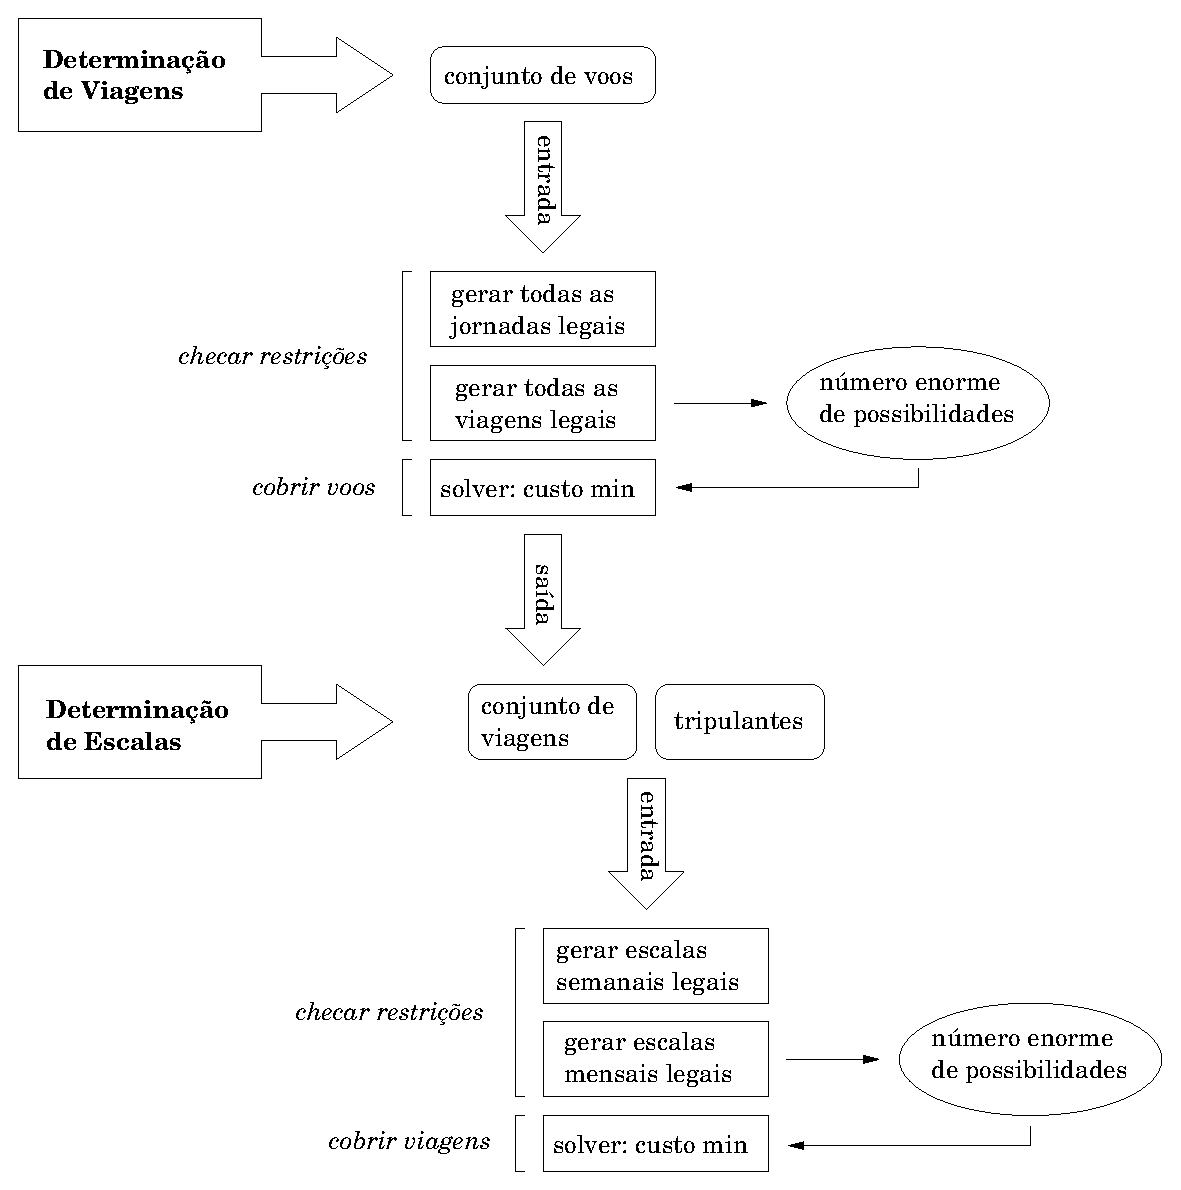
\includegraphics[scale=0.5]{fig/escalonamento.eps}
		\caption{Subproblemas enfrentados na solução do problema de escalonamento de tripulantes 
		(adaptado de~\cite{souai09}).}
		\label{fig:escalonamento}
	\end{center}
\end{figure}

%%%%%%%%%%%%%%%%%%%%%%%%%%%%%%%%%%%%%%%%%%%%%%%%%%%%%%%%%%%%%%%%%%%%%%%%%%%%%%%%%%%%%%%%%%%%%%%%%%%%

\section{Definições}
\label{sec:definicoes}

Antes que possamos apresentar e explorar a estrutura do problema com mais detalhes, faz-se
necessário a introdução de algumas definições e nomenclaturas usuais, as quais serão amplamente
utilizadas neste trabalho.

\begin{itemize}
	\item {\bf Etapa:} é um voo único sem paradas, também chamado de {\bf perna}, {\bf trecho} ou 
	{\bf segmento de voo}.
	\item {\bf Jornada:} conjunto de uma ou mais etapas sequenciais, também chamado de {\bf jornada 
	de trabalho}. 
	\item {\bf Tempo Mínimo de Conexão:} menor intervalo possível de tempo entre duas etapas 
	consecutivas em uma jornada.
	\item {\bf Tempo Máximo de Conexão:} maior intervalo possível de tempo entre duas etapas 
	consecutivas em uma jornada.
	\item {\bf Tempo de Briefing:} tempo mínimo que antecede o início da primeira etapa de uma
	jornada, necessário para o {\it briefing} da tripulação.
	\item {\bf Tempo de Debriefing:} tempo mínimo que sucede o término da último etapa de uma
	jornada, necessário para o {\it debriefing} da tripulação.
	\item {\bf Início da Jornada:} horário em que a tripulação deve apresentar-se para o início
	de uma jornada. Corresponde ao horário da decolagem da primeira etapa menos o tempo de 
	{\it briefing}. 
	Também chamado de {\bf checkin}.
	\item {\bf Término da Jornada:} horário em que a tripulação encerra suas atividades em uma 
	jornada. Corresponde ao horário de pouso da última etapa mais o tempo de {\it debriefing}.
	Também chamado de {\bf checkout}.
	\item {\bf Base Contratual:} cidade onde um dado tripulante está domiciliado, também
	chamada simplesmente de {\bf base}.
	\item {\bf Viagem:} conjunto de jornadas de trabalho, com a primeira etapa da primeira
	jornada e a última etapa da última jornada começando e terminando respectivamente na mesma
	base contratual. Uma viagem também é chamada de {\bf pairing}, ou {\bf rotação}.
	\item {\bf Descanso:} intervalo mínimo de tempo ininterrupto de repouso após uma jornada.
	\item {\bf Pernoite:} intervalo de tempo separando duas jornadas consecutivas de uma viagem.
\end{itemize}

A Figura~\ref{fig:viagem} apresenta o exemplo de uma viagem que ilustra alguns dos conceitos
expostos acima. As etapas na figura estão representadas pelos retângulos mais internos. São
indicados os aeroportos de origem e destino, bem como os horários de decolagem e pouso. As
jornadas são indicadas pelos retângulos pontilhados, englobando uma cadeia de etapas. A base 
contratual considerada é CGH (São Paulo). 

\begin{figure}[htbp]
	\begin{center}
		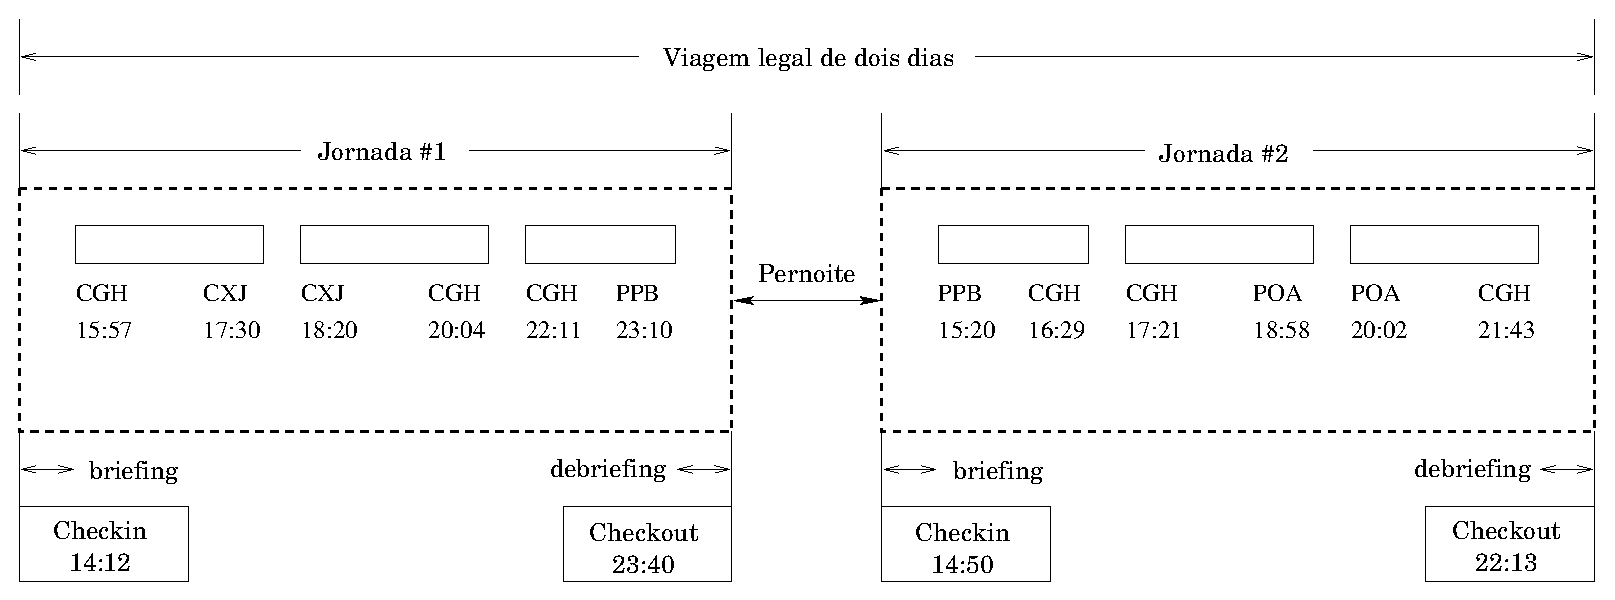
\includegraphics[scale=0.5]{fig/viagem.eps}
		\caption{Exemplo de uma viagem de dois dias para a base CGH.}
		\label{fig:viagem}
	\end{center}
\end{figure}

%%%%%%%%%%%%%%%%%%%%%%%%%%%%%%%%%%%%%%%%%%%%%%%%%%%%%%%%%%%%%%%%%%%%%%%%%%%%%%%%%%%%%%%%%%%%%%%%%%%%

\section{Formulação do PDV}
\label{sec:formulacao}

No problema da determinação das viagens, tem-se como entrada o conjunto de voos a ser operado pela
empresa, o conjunto de bases contratuais dos tripulantes, as regras de trabalho que ditam a
construção de viagens válidas e uma estrutura de custo (mais detalhes na
Seção~\ref{sec:regras_e_custos}). A saída, então, deve ser um conjunto de viagens que cubra todos os
voos operados exatamente e uma vez e que tenha o custo mínimo (veja Figura~\ref{fig:pdv}).

\begin{figure}[htbp]
	\begin{center}
		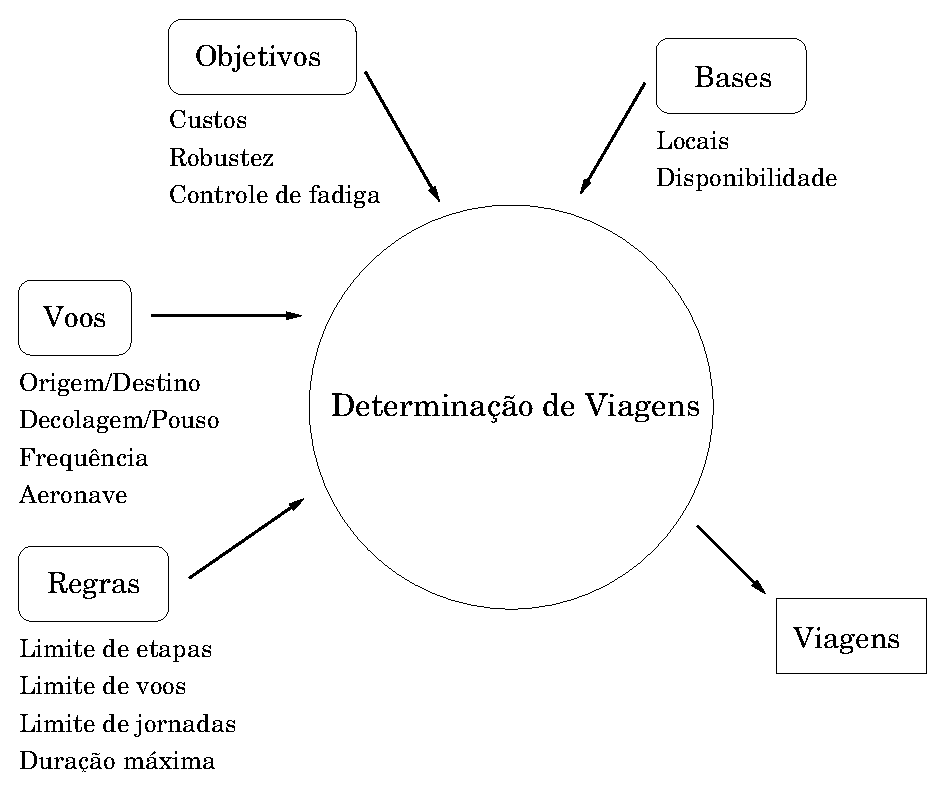
\includegraphics[scale=0.5]{fig/pdv.eps}
		\caption{Representação do problema da determinação de viagens (PDV).}
		\label{fig:pdv}
	\end{center}
\end{figure}

Normalmente os voos das companhias aéreas apresentam uma frequência regular de oferecimento, sendo
que a maioria deles operam diariamente. Outros são oferecidos apenas em alguns dias fixos da semana
e poucos são oferecidos vez ou outra no mês. Costuma-se então inicialmente resolver o problema
diário, onde se assume que todos os voos são repetidos diariamente. Note que, para o problema
diário, viagens de vários dias com etapas repetidas são inviáveis. Um segmento de voo repetido
causaria o efeito de mais de uma tripulação ser atribuída para realização dessa etapa, uma vez que
quando se faz a implementação da solução diária, uma tripulação distinta é atribuída a cada um dos
dias da viagem.

O problema semanal é mais complicado porque envolve um maior número de etapas consideradas. De
qualquer forma, a solução do problema semanal pode ser obtida a partir de um ajuste da solução do
problema diário, sem perda significativa de custo~\cite{gopalakrishnan05}. A solução do problema
mensal completo segue da solução do problema semanal. Como a maior parte da redução de custos está
associada à resolução do problema diário, ele torna-se o mais importante. Daqui em diante trataremos
apenas do problema diário.

Uma outra simplificação do problema está no fato de que os tripulantes são habilitados para operar
apenas um tipo, ou família, de aeronaves dentro de uma frota. Assim, fatora-se o problema da
determinação das viagens por tipo de aeronave. Para cada tipo, resolve-se um PDV considerando apenas
as etapas operadas por ele. No PDE, as viagens assim geradas são atribuídas apenas a tripulantes
habilitados a operar cada tipo de aeronave.

Há uma formulação natural para o PDV em termos de um problema de programação linear. Suponha que
seja possível gerar e enumerar todas as $n$ viagens associadas a uma dada entrada do problema
contendo $m$ etapas a serem cobertas. Seja $x_j \in \{0, 1\}$ uma variável de decisão que assume o
valor 1 se a viagem $j$ for escolhida na solução de custo mínimo e 0 caso contrário. Então, o PDV
pode ser modelado da seguinte forma:
%
\begin{eqnarray} \label{eq:sppv}
	\text{minimizar} && \displaystyle \sum_{j=1}^n c_j x_j \nonumber \\
	\text{sujeito à} && \displaystyle \sum_{j=1}^n a_{ij} x_j = 1 \ev \;\; i = 1, \ldots, m \\
		               && x_j \in \{0, 1\} \ev \;\; j = 1, \ldots, n \ep \nonumber
\end{eqnarray} 
%
Os coeficientes $a_{ij}$ são definidos por (matriz de incidência)
%
\begin{equation*}
	a_{ij} = \left\{
	\begin{array}{ll}
			1 \ev & \text{se a viagem $j$ cobre a etapa $i$} \\
			0 \ev & \text{caso contrário}
	\end{array}
	\right.
\end{equation*}

As restrições em (\ref{eq:sppv}) garantem que cada etapa seja coberta exatamente uma vez por alguma
viagem. Existe ainda uma formulação alternativa onde as restrições são dadas por
%
\begin{equation} \label{eq:dh} 
	\sum_{j=1}^n a_{ij} x_j \geq 1 \, , \;\; i = 1, \ldots, m \ep
\end{equation} 
%
Nesse caso uma mesma etapa pode ser coberta por mais de uma viagem e o problema passa a ser
denominado \emph{set cover}. Do ponto de vista do escalonamento, se uma etapa é coberta por mais
de uma viagem, então uma tripulação estará trabalhando nessa etapa e as demais viajando de
passageiro (situação conhecida por \emph{deadheading}). Às vezes, essa situação é necessária para
que se garanta a viabilidade da solução. Se o preço a se pagar pela operação com \emph{deadheading} 
for essencialmente o mesmo de uma operação normal, então não há alteração significativa no custo 
da viagem associada. Isso permite que o problema seja modelado com as restrições (\ref{eq:dh}) 
sem alterar a estrutura de custos.

É comum a inserção de restrições adicionais ao modelo que garantem uma distribuição de trabalho
entre as bases compatível com os recursos disponíveis em cada uma. Se o número total de bases do
problema considerado é $r$, então as \emph{restrições de bases} são expressas por
%
\begin{equation} \label{eq:bases}
	H_k^L \leq \sum_{j=1}^n h_{kj} x_j \leq H_k^U \, , \;\; k = 1, \ldots, r \ev
\end{equation}
%
onde $H_k^L$ é o número mínimo de horas disponíveis na base $k$ e $H_k^U$ é seu número máximo. 
Note que $H_k^L$ pode ser diferente de zero desde que se exija que não mais do que um certo número 
de tripulantes fique de reserva. O coeficiente $h_{kj}$ dá o número de horas necessárias para 
efetuar a viagem $j$ ($h_{kj} = 0$ se a viagem $j$ não pertencer à base $k$).

O grande problema com a formulação (\ref{eq:sppv}) está no enorme número de variáveis geradas, mesmo
nos casos das instâncias pequenas (poucas etapas diárias). A Tabela~\ref{tab:viagens} ilustra o
número de viagens válidas geradas, com duração máxima de 3 ou 4 dias, para diversas frotas de
aeronaves. O número enorme de variáveis está associada com a natureza combinatória do problema. A
maioria das empresas aéreas operam em aeroportos conhecidos como \emph{hubs}, onde um grande número
de aeronaves chegam e partem em um mesmo intervalo de tempo, possibilitando que os passageiros
efetuem suas conexões para uma variedade de destinos em pouco tempo. Esse tipo de estrutura em rede 
leva à explosão no número de viagens válidas que podem ser construídas~\cite{graves93}. Note na
Tabela~\ref{tab:viagens} que, apesar do número de viagens ser gigantesco, o número de 
jornadas tem um valor mais gerenciável.

\begin{table}[ht]
	\begin{center}
		\begin{tabular}{|c||c|c|c|c|c|}
			\hline
			{\bf Frota} & {\bf Max Dias} & {\bf Etapas} & {\bf Bases} & {\bf Jornadas} & 
			{\bf Viagens} ($\times 10^6$) \\
			\hline
			AAS80 & 3 & 1.152 & 12 & 690.000 & 48.400 \\
			\hline
			AA757 & 3 & 251 & 15 & 7.000 & 1 \\
			\hline
			AA727 & 3 & 375 & 11 & 31.000 & 36 \\
			\hline
			AAF10 & 4 & 307 & 3 & 55.000 & 63.200 \\
			\hline 
			UA737 & 4 & 773 & 7 & 568.000 & 100.000.000 \\
			\hline
			USDC9 & 4 & 478 & 4 & 562.000 & 105.000.000 \\
			\hline
		\end{tabular}
		\caption{Jornadas e viagens válidas geradas para um conjunto de frotas de aeronaves
		de companhias norte-americanas (fonte:~\cite{anbil98}).}
		\label{tab:viagens}
	\end{center}
\end{table}

Como o problema de partição é NP-difícil~\cite{garey79}, a aplicação de métodos diretos de
otimização é impraticável para qualquer situação real. Discutiremos esse ponto na
Seção~\ref{sec:preliminar}. Os métodos de solução normalmente envolvem algum tipo de heurística e/ou
algum critério de parada que leva a soluções sub-ótimas.

%%%%%%%%%%%%%%%%%%%%%%%%%%%%%%%%%%%%%%%%%%%%%%%%%%%%%%%%%%%%%%%%%%%%%%%%%%%%%%%%%%%%%%%%%%%%%%%%%%%%

\section{Objetivos e Estrutura}
\label{sec:objetivos}

Neste trabalho focamos no problema da determinação das viagens. Os objetivos foram estudar a 
literatura, entender e implementar alguns dos métodos de solução disponíveis, aplicando-os
no contexto de companhias aéreas brasileiras e, por fim, analisar os resultados obtidos.

O contexto brasileiro difere significativamente dos contextos estrangeiros no que refere-se à 
estrutura de custos e regras que ditam a viabilidade de uma viagem. Como os trabalhos estudados na
literatura referem-se ao escopo norte-americano e europeu, tivemos por objetivo também efetuar as 
devidas adaptações na tentativa de solucionar problemas de companhias aéreas brasileiras.

Esta monografia está estruturada da seguinte forma: neste capítulo faz-se uma introdução e
contextualização do problema em estudo. Em seguida, no Capítulo~\ref{cap:geracao}, apresentamos o
método de geração de viagens, com destaque especial na estrutura de custos e regras de viabilidade,
e um exemplo explícito é apresentado. No Capítulo~\ref{cap:heuristicas}, apresentamos as três
heurísticas implementadas neste trabalho, a saber, um método de busca local, um algoritmo genético
híbrido e um procedimento de geração de colunas. O Capítulo~\ref{cap:resultados} mostra os
resultados obtidos aplicando-se as heurísticas estudadas a algumas instâncias reais do problema. Em
particular, mostramos a redução do custo da solução em função do número de iterações que controla a
evolução dos algoritmos. Finalmente, no Capítulo~\ref{cap:conclusao}, destacamos algumas conclusões
e comparações de resultados. Listamos também alguns pontos de melhorias, dificuldades com o projeto
e perspectivas futuras.

A segunda parte desta monografia apresenta o conteúdo subjetivo, destacando a opinião e as
impressões de cada autor sobre o curso do BCC/IME e sua relação com este projeto
(Capítulo~\ref{cap:analise_subjetiva}).